\chapter{固有距離、克魯斯卡爾幾何與視界觀察者}

史瓦西度規在視界處似乎變得奇異，但曲率並非如此。為了區分這兩種說法，我們先消去黑洞的整體尺度，再以距視界的固有距離取代徑向座標。在視界附近，所得幾何就是以加速座標表示的普通平直時空。畫出這種幾何後，關於 Alice、Bob 和 Charlie 的問題就成了世界線與光線的問題，不再是言語上的悖論。

\section{消去史瓦西半徑的尺度}

先從帶撇號的座標開始，讓重新縮放後的變數稍後能使用熟悉的名稱：
\begin{equation}
d\tau^2
=
\left(1-\frac{2MG}{r'}\right)dt'^2
-
\frac{dr'^2}{1-\frac{2MG}{r'}}
-
r'^2d\Omega_2^2.
\label{eq:l7-schwarzschild-dimensional}
\end{equation}
引入史瓦西半徑與無量綱座標
\begin{equation}
r_{\mathrm S}=2MG,
\qquad
r=\frac{r'}{r_{\mathrm S}},
\qquad
t=\frac{t'}{r_{\mathrm S}}.
\label{eq:l7-rescaling}
\end{equation}
我們取 \(c=1\)，因此時間和長度使用相同的單位。半徑 \(r_{\mathrm S}\) 因而既是長度，也是光穿越該長度所需的時間。代入後得到
\begin{equation}
d\tau^2
=r_{\mathrm S}^2
\left[
\left(1-\frac1r\right)dt^2
-
\frac{dr^2}{1-\frac1r}
-
r^2d\Omega_2^2
\right].
\label{eq:l7-schwarzschild-rescaled}
\end{equation}
因此，所有不旋轉、不帶電的史瓦西黑洞都有相同的無量綱幾何。改變質量會改變乘在度規前的尺度因子，卻不改變方括號內的形式。這就像把球的每個距離都除以球半徑後再畫出來：同一幅圖可以描述月球和地球，雖然圖上的一公分在兩種情況下代表不同的物理距離。

\begin{classroomqa}
\audiencequestion{度規的徑向部分與角向部分各自帶什麼符號？}
\lecturerresponse{採用本書所用的 \(+---\) 符號慣例時，兩個空間部分都帶負號。寫下這個式子時，課堂上有人當場指出了符號。角向因子可以用正弦或餘弦，取決於極座標是從軸線還是赤道量起；使用簡潔記號 \(d\Omega_2^2\) 就能避開這項慣例上的差異。
\lecturetimestamp{00:07:48--00:08:12}}
\end{classroomqa}

\section{視界處的曲率尺度}

不必進行冗長的張量計算，這種重新縮放就能回答一個重要的物理問題。度規分量是無量綱的。克里斯托費爾符號含有一個座標導數，因此量綱為長度的倒數；黎曼張量在物理正交標架中的分量則具有以下量綱
\begin{equation}
[g_{\mu\nu}]=1,
\qquad
[\Gamma^\mu{}_{\nu\rho}]=L^{-1},
\qquad
[R_{\hat\alpha\hat\beta\hat\gamma\hat\delta}]
=L^{-2}.
\label{eq:l7-curvature-dimensions}
\end{equation}
在視界 \(r=1\) 處，唯一可用的物理長度是 \(r_{\mathrm S}\)。因此，潮汐曲率的尺度必定是
\begin{equation}
\left|R_{\hat\alpha\hat\beta\hat\gamma\hat\delta}\right|_{\mathrm{hor}}
\sim \frac{1}{r_{\mathrm S}^2}.
\label{eq:l7-horizon-curvature}
\end{equation}
更一般地說，它等於 \(r_{\mathrm S}^{-2}\) 乘上一個 \(r\) 的無量綱函數。這裡談的是黎曼張量所描述的潮汐場，而不是在史瓦西真空中為零的里奇純量。

物理結論立刻就很清楚：質量增加會使 \(r_{\mathrm S}\) 增大，並減弱視界處的潮汐場。小黑洞可能在延展物體穿越視界時將它撕裂；超大質量黑洞的視界附近，潮汐力則可能很弱。不過，曲率會隨著向內深入而增大，並在 \(r=0\) 發散。因此，視界和奇異點是截然不同的對象。

\section{距視界的固有距離}

接下來的局部計算都令 \(r_{\mathrm S}=1\)。在相對論中，座標變換並非表面上的修飾：不恰當的座標可能讓規則的幾何隱藏在奇異的係數背後。史瓦西座標差 \(r-1\) 並不是從視界量起的徑向距離。

\begin{figure}[htbp]
\centering
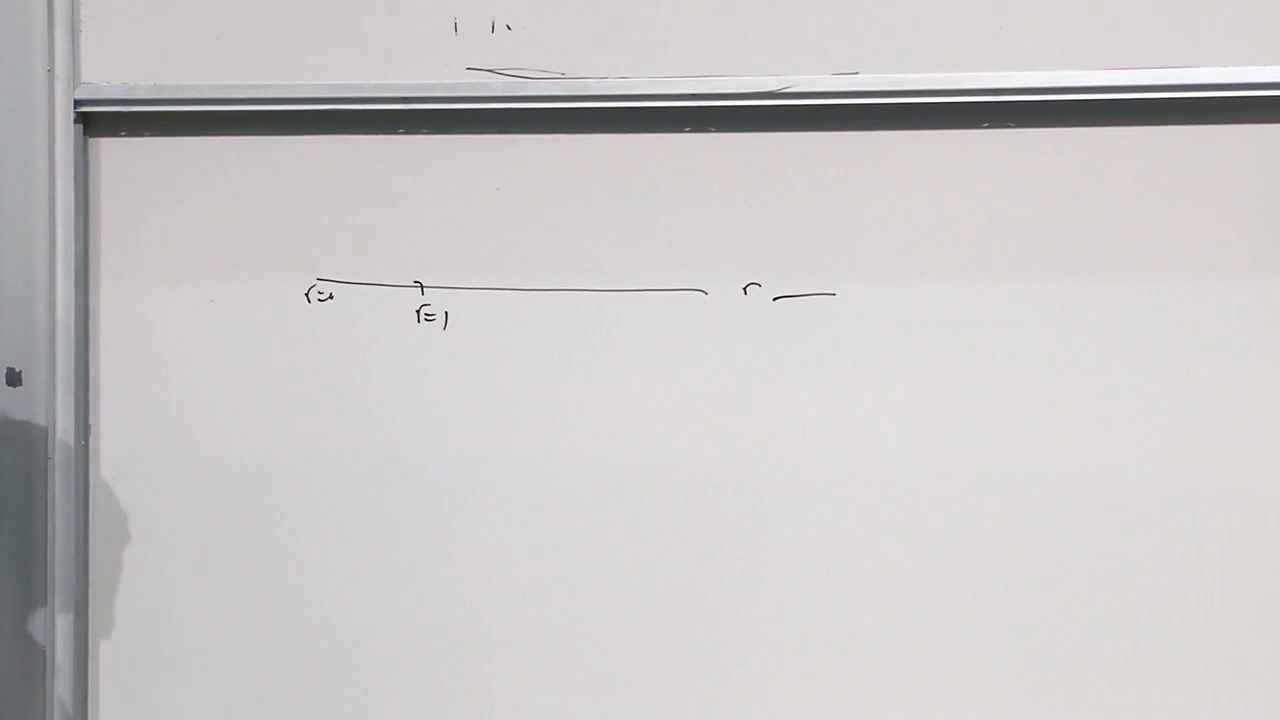
\includegraphics[width=0.78\textwidth]{lecture_07_figure_02.png}
\caption{黑板上使用的徑向座標線。視界位於 \(r=1\)，而 \(r=0\) 是曲率奇異點。}
\lectureframe{00:16:11}
\end{figure}

固定 \(t\) 和角度不變。此時正的空間線元素為
\begin{equation}
ds^2=\frac{dr^2}{1-\frac1r},
\qquad
ds=\sqrt{\frac{r}{r-1}}\,dr.
\label{eq:l7-radial-proper-line}
\end{equation}
以下式定義距視界的無量綱固有距離：
\begin{equation}
\rho(r)
=
\int_1^r\sqrt{\frac{r'}{r'-1}}\,dr'.
\label{eq:l7-rho-definition}
\end{equation}
恢復整體尺度後，物理距離為 \(r_{\mathrm S}\rho\)。我們不需要這個積分的閉合形式，只需要它的導數：
\begin{equation}
\frac{d\rho}{dr}
=\sqrt{\frac{r}{r-1}},
\qquad
d\rho^2
=\frac{dr^2}{1-\frac1r}.
\label{eq:l7-rho-derivative}
\end{equation}
於是，複雜的徑向項恰好化為 \(-d\rho^2\)。這正是引入 \(\rho\) 的原因。

接著再縮放一次時間座標，
\begin{equation}
\omega=\frac{t}{2}.
\label{eq:l7-omega}
\end{equation}
由於 \(r\) 是 \(\rho\) 的函數，度規可以寫成
\begin{equation}
d\tau^2
=
F(\rho)\rho^2d\omega^2
-
d\rho^2
-
r(\rho)^2d\Omega_2^2.
\label{eq:l7-rho-metric}
\end{equation}

\begin{classroomqa}
\audiencequestion{\(F(\rho)\) 是否只是為了把時間係數寫成 \(F(\rho)\rho^2\) 的形式而定義的？}
\lecturerresponse{是的。此時這個因式分解並沒有獨立的物理意義，只是為了方便而作的定義。等到考察 \(F\) 在視界附近與遠處的極限時，它的用處就顯現出來了。
\lecturetimestamp{00:26:39--00:26:59}}
\end{classroomqa}

在遠處，史瓦西時間係數趨近於一。由於 \(dt=2d\omega\)，便得到
\begin{equation}
\lim_{\rho\to\infty}F(\rho)\rho^2=4.
\label{eq:l7-far-limit}
\end{equation}
在視界附近，式~\eqref{eq:l7-rho-definition}給出
\begin{equation}
\begin{aligned}
\rho&\simeq 2\sqrt{r-1},\\
r(\rho)&=1+\frac{\rho^2}{4}+O(\rho^4),\\
\lim_{\rho\to0}F(\rho)&=1.
\end{aligned}
\label{eq:l7-near-expansion}
\end{equation}

\begin{figure}[htbp]
\centering
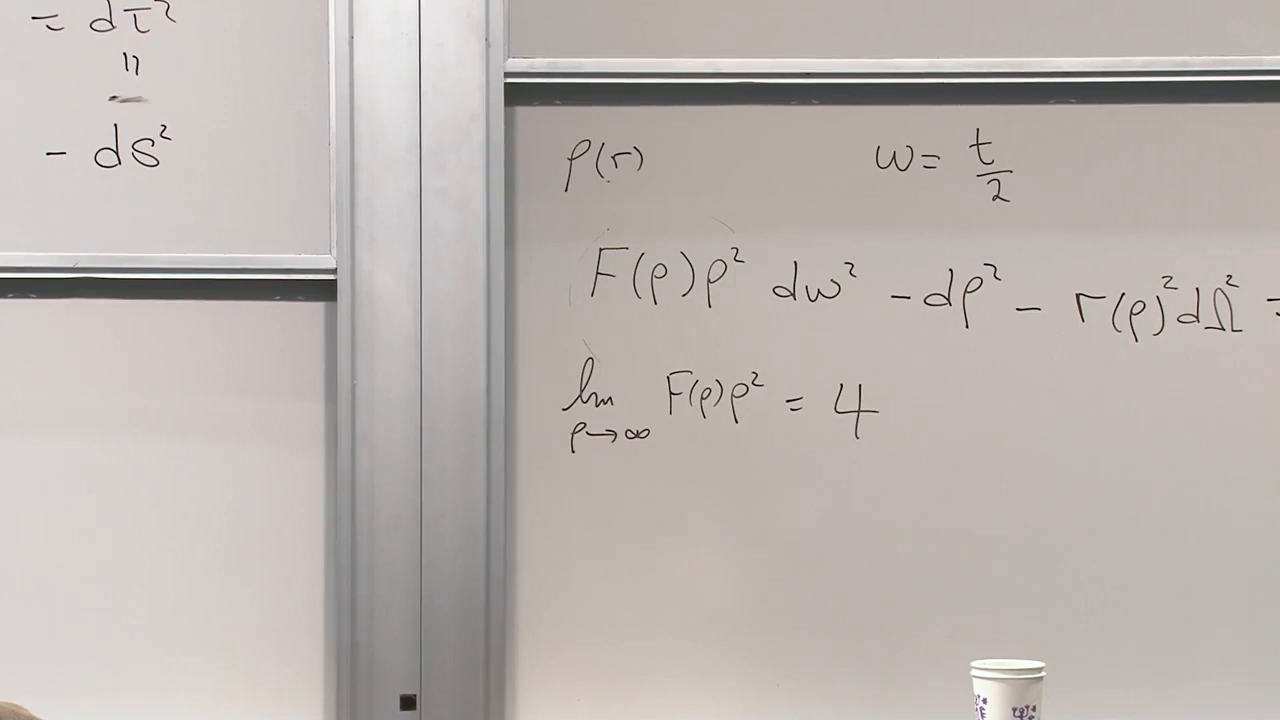
\includegraphics[width=0.90\textwidth]{lecture_07_figure_03.png}
\caption{\((\rho,\omega)\)座標中的度規、其漸近時間係數，以及近視界極限\(F\to1\)和\(r=1+\rho^2/4+\cdots\)。}
\lectureframe{00:37:30}
\end{figure}

\section{視界處隱藏的平直時空}

在\(\rho=0\)附近，式~\eqref{eq:l7-rho-metric}的徑向—時間部分化為
\begin{equation}
d\tau_{\mathrm{radial}}^2
\simeq
\rho^2d\omega^2-d\rho^2.
\label{eq:l7-rindler-metric}
\end{equation}
這是以雙曲極座標表示的平直閔考斯基時空。定義
\begin{equation}
X=\rho\cosh\omega,
\qquad
T=\rho\sinh\omega.
\label{eq:l7-rindler-transform}
\end{equation}
於是
\begin{equation}
dT^2-dX^2
=
\rho^2d\omega^2-d\rho^2.
\label{eq:l7-minkowski-check}
\end{equation}
固定 \(\rho\) 的曲線滿足
\begin{equation}
X^2-T^2=\rho^2
\label{eq:l7-constant-rho}
\end{equation}
因此是雙曲線。固定 \(\omega\) 的曲線則是從原點出發的射線。當 \(\omega\to\infty\) 時，這些射線趨近零線 \(T=X\)。因此，在正則圖中，表面上被放逐到無限座標時間的史瓦西視界，其實只是一條普通的零線。

\begin{figure}[htbp]
\centering
\includegraphics[width=0.88\textwidth]{lecture_07_figure_06.png}
\caption{完整的黑板幾何：固定\(\rho\)的雙曲線、固定\(\omega\)的射線、零視界，以及視界上方的\(r<1\)區域。}
\lectureframe{00:38:30}
\end{figure}

\begin{figure}[htbp]
\centering
\resizebox{0.96\linewidth}{!}{%
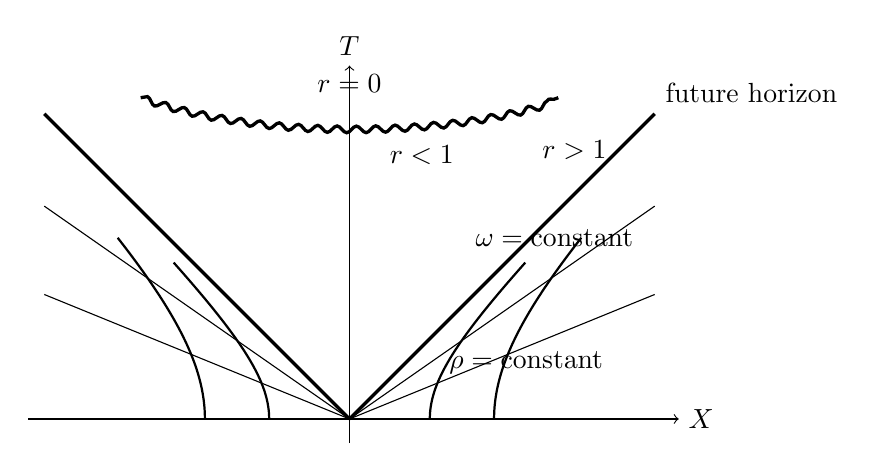
\begin{tikzpicture}[scale=1.02]
\draw[->] (-4.0,0) -- (4.1,0) node[right] {$X$};
\draw[->] (0,-0.3) -- (0,4.4) node[above] {$T$};
\draw[very thick] (0,0) -- (3.8,3.8)
  node[above right] {future horizon};
\draw[very thick] (0,0) -- (-3.8,3.8);
\draw[thick]
  plot[domain=0:1.42,samples=50]
  ({1.0*cosh(\x)},{1.0*sinh(\x)});
\draw[thick]
  plot[domain=0:1.05,samples=50]
  ({1.8*cosh(\x)},{1.8*sinh(\x)});
\draw[thick]
  plot[domain=0:1.42,samples=50]
  ({-1.0*cosh(\x)},{1.0*sinh(\x)});
\draw[thick]
  plot[domain=0:1.05,samples=50]
  ({-1.8*cosh(\x)},{1.8*sinh(\x)});
\draw[thin] (0,0) -- (3.8,1.55);
\draw[thin] (0,0) -- (3.8,2.65);
\draw[thin] (0,0) -- (-3.8,1.55);
\draw[thin] (0,0) -- (-3.8,2.65);
\draw[very thick,decorate,decoration={snake,amplitude=1.2pt,segment length=7pt}]
  (-2.6,4.0) .. controls (-1.2,3.5) and (1.2,3.5) .. (2.6,4.0);
\node at (0,4.18) {$r=0$};
\node at (2.2,0.7) {$\rho=\mathrm{constant}$};
\node at (2.55,2.25) {$\omega=\mathrm{constant}$};
\node at (0.9,3.28) {$r<1$};
\node at (2.8,3.35) {$r>1$};
\end{tikzpicture}
}
\caption{清楚重建出的因果結構。視界是一條零線，而曲率奇異點\(r=0\)是黑洞內部的未來邊界。}
\label{fig:l7-kruskal-clean}
\end{figure}

小\(\rho\)極限不同於歐幾里得極座標中的小半徑極限。小的歐幾里得圓會收縮成一點；固定\(\rho\)的雙曲線則會趨近整條零線。因此，\(\rho=0\)標記的是整個視界，而不只是座標軸的交點。

外部的公式可以解析延拓至\(r<1\)。在視界附近，\(r-1\simeq\rho^2/4\)，因此內部形式上對應於\(\rho^2<0\)。可以把\(\rho\)稱為虛數，但更簡潔的做法是使用\(\rho^2\)、\(r\)或正則座標\(T,X\)。在內部，史瓦西\(t\)與\(r\)係數的符號互換。這不表示物理手錶變成了尺；而是表示史瓦西座標交換了因果性質。

\begin{classroomqa}
\audiencequestion{視界內部的水平雙曲線是什麼？直線射線又代表什麼？}
\lecturerresponse{雙曲線是延拓至\(r<1\)內的固定\(r\)曲線，也就是固定\(\rho^2\)的曲線。射線則是固定史瓦西時間的曲線。在外部，它們構成一個實用的座標網格；在內部，不能把相同的標記誤認為物理觀察者的軌跡。
\lecturetimestamp{00:44:12--00:44:59}}
\end{classroomqa}

\begin{classroomqa}
\audiencequestion{垂直方向是時間座標嗎？它代表哪個參考系？}
\lecturerresponse{它是新時空圖中的正則時間方向，但不是奇異的史瓦西時間\(t\)。這張圖配合的是自由落體的因果結構。固定在外部某個半徑的觀察者沿雙曲線運動，必須有加速度；自由落體的觀察者則會平順地穿越零視界。
\lecturetimestamp{00:45:54--00:46:48}}
\end{classroomqa}

\begin{classroomqa}
\audiencequestion{如果內部有\(\rho^2<0\)，那麼明確的\(i\)因子在哪裡？}
\lecturerresponse{可以引入虛數\(\rho\)，但這麼做沒有益處。不變的物理內容由\(r\)、\(\rho^2\)以及實數的正則座標\(T,X\)承載。關係式\(r-1\simeq\rho^2/4\)只是在視界附近成立的展開式。
\lecturetimestamp{00:52:35--00:53:00}}
\end{classroomqa}

講座中常把這張正則圖稱為克魯斯卡爾圖。嚴格來說，精確的克魯斯卡爾座標還包含一個徑向因子，使完整的史瓦西度規保持正則；式~\eqref{eq:l7-rindler-transform}則是它的近視界形式。因果上的訊息相同：視界是平滑的，但黑洞內每一條未來指向的類時曲線或零曲線，最終都會終止於\(r=0\)。沒有任何超光速的轉向能讓它穿越視界返回外部。

\subsection{如何理解座標奇異性}

由於原始的史瓦西座標讓視界處的係數看起來奇異，因此在歷史上，人們很難看出視界其實是平滑的。愛丁頓以及後來的芬克爾斯坦引入了能穿越視界的座標；芬克爾斯坦也辨認出這是一個單向的因果邊界。克魯斯卡爾憑藉他在電漿物理中累積的座標變換本領，為永恆解提供了全域正則的圖像。

接著，講座稍作停留，談到約翰・惠勒（John Wheeler）如何讓「黑洞」一詞變得無可迴避。這段談話既關乎個人，也關乎歷史：即使惠勒與人對政治議題有尖銳歧見，包括對核武競爭的看法，他仍被記得是一位溫和、深思熟慮的朋友。講者講了一則幽默的個人軼事，以免把惠勒刻畫成拘泥社交常規的人。技術上的討論則以「黑洞無毛」這句反駁重新接上。受到擾動的非旋轉黑洞會迅速趨於球對稱；旋轉黑洞則會趨於由其守恆參數決定的定常形狀。這是講座對無毛概念的定性說明，並非完整定理的證明。

\section{愛麗絲穿越視界；鮑勃留在外部}

最大延拓圖中有些區域，不會出現在由普通初始條件下恆星坍縮形成的簡單時空中。討論觀察者實驗時，我們只用到外部、未來視界與黑洞內部。

\begin{figure}[htbp]
\centering
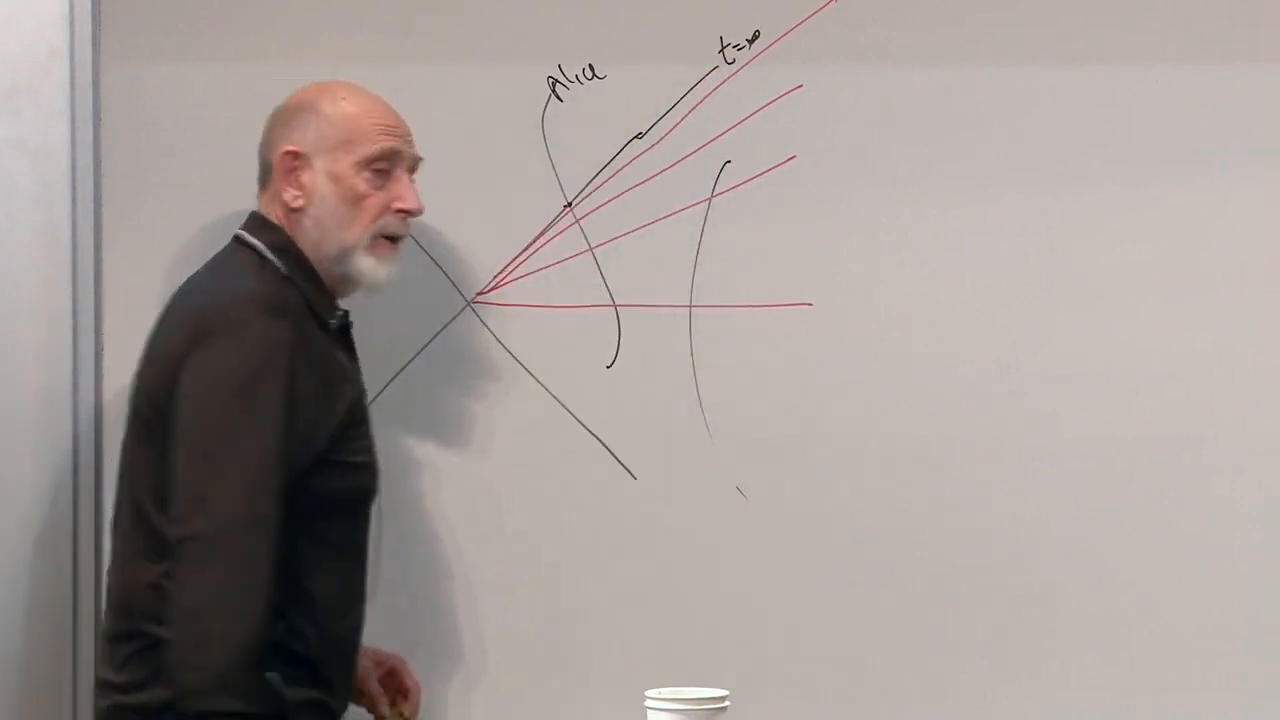
\includegraphics[width=0.84\textwidth]{lecture_07_figure_04.png}
\caption{愛麗絲的下落世界線，以及固定史瓦西時間的射線。極限射線標記為\(t=\infty\)。}
\lectureframe{00:54:54}
\end{figure}

愛麗絲自由落下。她的世界線會穿越視界，並在有限的固有時間內抵達奇異點。如果黑洞夠大，使視界處的潮汐力很小，那麼她的時鐘在穿越視界時不會發生任何異常。

鮑勃則停留在固定的外部半徑。要維持在那個位置，他必須加速。愛麗絲軌跡上較晚時刻發出的光抵達鮑勃時，延遲越來越長，紅移也越來越大。用史瓦西時間描述時，愛麗絲會趨近\(t=\infty\)；她穿越視界後發出的訊號，鮑勃永遠收不到。這些說的是因果訊號和外部切片，並不表示視界處有一層物質表面。

\begin{classroomqa}
\audiencequestion{如果鮑勃看到愛麗絲變慢，愛麗絲是否就會看到鮑勃變快？}
\lecturerresponse{不會。只要愛麗絲的世界線還在延續，她就會持續收到鮑勃發出的普通光訊號。鮑勃的世界線上有一個最後能傳訊給她的事件；之所以是最後一個，只是因為愛麗絲隨後就會撞上奇異點。鮑勃身上並沒有發生什麼突然的變化。觀察總是仰賴過去光錐，而這兩條世界線之間的因果關係並不對稱。
\lecturetimestamp{00:58:31--01:01:23}}
\end{classroomqa}

\begin{classroomqa}
\audiencequestion{如果在鮑勃的座標中，愛麗絲仍然靠近視界，他能不能下去救她，再返回外部？}
\lecturerresponse{救援者的世界線必須在愛麗絲穿越事件視界之前與她相遇。穿越之後，就沒有任何未來指向的路徑能再與她相遇並返回外部。史瓦西切片把穿越時刻放在\(t=\infty\)，但這不表示愛麗絲停留在一個可以救回的物質表面上；這表示這些切片無法提供一個跨越視界的全域「現在」概念。
\lecturetimestamp{01:01:24--01:02:12}}
\end{classroomqa}

\section{查理跟隨愛麗絲}

讓查理在愛麗絲後方不遠處落下。如此一來，兩人在視界附近都近似作慣性運動。他們可以交換訊號、雙向交談，甚至牽手。兩人都不會看到標示視界的路牌。這裡與鮑勃的差異，不在於三個人的身分，而在於自由落體和留在外部的加速世界線有所不同。

\begin{classroomqa}
\audiencequestion{如果愛麗絲先落下，查理像籃球跟著籃框一樣跟在後面，鮑勃會看到什麼？}
\lecturerresponse{鮑勃會看到兩人都逐漸接近視界。愛麗絲在前方，因此會先顯得逐漸變慢，並在徑向上受到壓縮。查理看來越來越接近她，但在鮑勃的極限外部視角中，始終追不上她。這種視覺上的堆積，並非兩位自由落體者實際感受到的情況。
\lecturetimestamp{01:04:12--01:06:05}}
\end{classroomqa}

\begin{classroomqa}
\audiencequestion{表觀上的壓扁是否與潮汐力相矛盾？潮汐力應該會沿徑向拉長自由落體者。}
\lecturerresponse{這是兩種不同的效應。壓扁是鮑勃以史瓦西座標描述時看到的現象；潮汐拉伸則是愛麗絲和查理能感受到的局部曲率效應。這裡討論觀察者時，假設黑洞夠大，或觀察者夠小，使視界處的潮汐效應可以忽略。質量約為太陽質量的黑洞，視界處的潮汐力會很猛烈；超大質量黑洞的視界潮汐力則可能很弱。
\lecturetimestamp{01:06:07--01:08:18}}
\end{classroomqa}

\begin{classroomqa}
\audiencequestion{查理還在外部時，能看到愛麗絲穿越視界嗎？}
\lecturerresponse{畫出那條零射線。愛麗絲穿越視界時發出的光會沿著視界傳播，並在查理穿越時抵達。到了那個事件，查理可以推知自己看到了她穿越視界；但兩人都不會在當地遇到任何標記。之後，查理可以看到她在內部。如果他在穿越前加速離開，並成功留在外部，就永遠看不到那次穿越。
\lecturetimestamp{01:08:19--01:11:11}}
\end{classroomqa}

\begin{classroomqa}
\audiencequestion{如果愛麗絲已在內部而查理仍在外部，該如何比較他們後來的半徑與穿越時刻？}
\lecturerresponse{「同一時間」這種說法，無法給出一種與觀察者無關的同時性關係。愛麗絲會在自己的過去光錐上看到查理；只有當她進入更深處後，才可能看到他後來穿越視界。具體的世界線和零射線才能回答這個問題。若要把情況推廣到許多相距遙遠的落體者，就必須畫出他們實際的因果圖來檢查，不能假設所有人都共用一個普遍的穿越時刻。
\lecturetimestamp{01:11:14--01:12:31}}
\end{classroomqa}

在正則的近視界座標中，自由落體軌跡近似直線。在完整的史瓦西幾何中，它並非完全筆直；不過在大型、曲率微弱的視界附近，這個近似相當好。

\begin{classroomqa}
\audiencequestion{弦理論能否解決黑洞內部量子重力區域會發生什麼事？}
\lecturerresponse{這正是問題變得微妙之處。奇異點附近需要量子重力理論；弦理論是一種候選架構，但當時相關問題仍在研究中，而且十分困難，並非只要簡單套用經典圖像就能解決。
\lecturetimestamp{01:13:04--01:13:38}}
\end{classroomqa}

\begin{classroomqa}
\audiencequestion{愛麗絲穿越視界時，她自己的時鐘和速度會怎樣？}
\lecturerresponse{她的時鐘會以平常的局部速率持續走動，並記錄有限的固有時間。在她當下的靜止系中，她處於靜止；相對於局部自由落體參考系，她具有一般而有限的速度。在大型黑洞的視界附近，幾何近乎平坦，因此她世界線上的等固有時間標記都保持規則，直到奇異點附近的曲率變得強烈。
\lecturetimestamp{01:13:39--01:14:44}}
\end{classroomqa}

\begin{classroomqa}
\audiencequestion{如果鮑勃向外加速，卻不夠快，還是掉進去了，會怎樣？}
\lecturerresponse{他的世界線會向外彎，但仍然穿越視界。如果他很晚才穿越，就能在愛麗絲穿越後不久看到她，但在抵達奇異點前所剩的固有時間很短。草圖上的世界線斜率不是經過校準的尺或鐘；真正保留下來的是因果順序，而不是圖上量得的歐幾里得長度。
\lecturetimestamp{01:14:47--01:16:31}}
\end{classroomqa}

所有這些結論都假設沒有訊號能超越光速。講座簡短地拿當時不久前的新聞報導開玩笑；報導聲稱義大利測得似乎超光速的中微子。這影射的是實驗計時誤差，並非相對論的例外。因果結構仍受零線所限制。

\begin{classroomqa}
\audiencequestion{如果愛麗絲和鮑勃帶著已同步的時鐘，而愛麗絲朝視界俯衝後又返回，能用這些時鐘判定問題嗎？}
\lecturerresponse{兩人相遇時可以比對時鐘；但世界線分開後，就不存在唯一的遠距同步方式，尤其是其中一人改變運動狀態時。畫出兩條世界線及彼此交換的零射線，就能針對指定的實驗得到可操作的答案。
\lecturetimestamp{01:17:34--01:18:25}}
\end{classroomqa}

\begin{figure}[htbp]
\centering
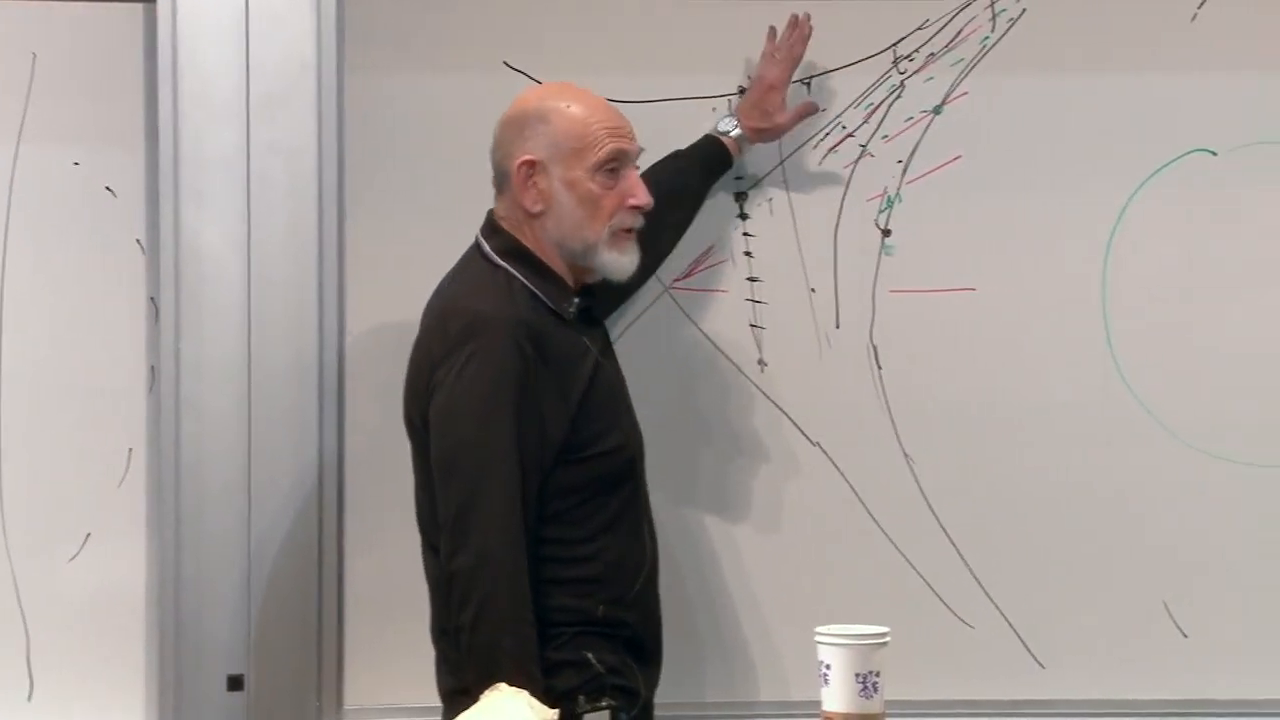
\includegraphics[width=0.86\textwidth]{lecture_07_figure_05.png}
\caption{用來回答愛麗絲、鮑勃和查理問題的累積因果圖。每次觀測的位置，都由一條從被觀測事件追蹤至觀察者世界線的零射線確定。}
\lectureframe{01:18:12}
\end{figure}

\begin{figure}[htbp]
\centering
\resizebox{0.96\linewidth}{!}{%
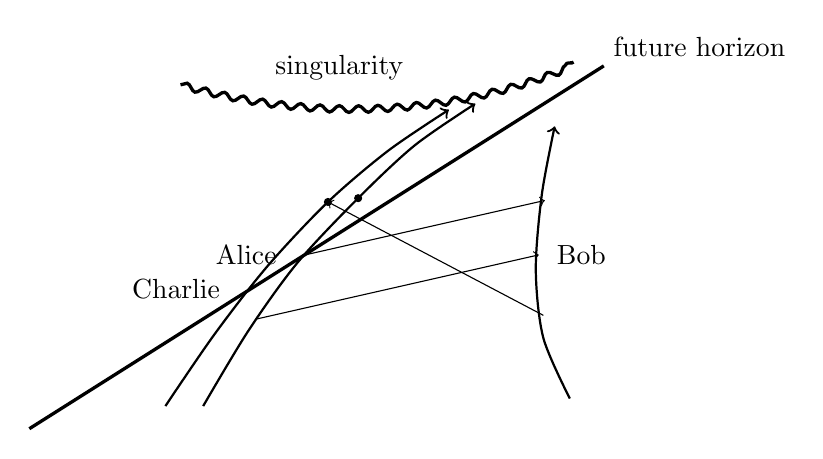
\begin{tikzpicture}[scale=0.96]
\draw[very thick] (-3.8,-0.3) -- (3.8,4.5);
\node[above right] at (3.8,4.5) {future horizon};
\draw[very thick,decorate,decoration={snake,amplitude=1.2pt,segment length=7pt}]
  (-1.8,4.25) .. controls (0.1,3.72) and (2.0,3.92) .. (3.4,4.55);
\node at (0.3,4.48) {singularity};
\draw[thick,->]
  plot[smooth] coordinates {(-1.5,0.0) (-0.9,1.0) (-0.25,1.9)
  (0.55,2.75) (1.3,3.45) (2.1,4.0)};
\node[left] at (-0.4,2.0) {Alice};
\draw[thick,->]
  plot[smooth] coordinates {(-2.0,0.0) (-1.35,0.95) (-0.65,1.85)
  (0.15,2.7) (0.95,3.38) (1.75,3.92)};
\node[left] at (-1.15,1.55) {Charlie};
\draw[thick,->]
  plot[smooth] coordinates {(3.35,0.1) (3.0,0.9) (2.9,1.8)
  (2.98,2.8) (3.15,3.7)};
\node[right] at (3.05,2.0) {Bob};
\draw[thin,->] (-0.8,1.15) -- (2.94,2.0);
\draw[thin,->] (-0.15,2.0) -- (3.02,2.72);
\draw[thin,->] (3.0,1.2) -- (0.15,2.7);
\draw[fill] (0.55,2.75) circle (1.3pt);
\draw[fill] (0.15,2.7) circle (1.3pt);
\end{tikzpicture}
}
\caption{觀察者示意圖。鮑勃在外部的觀測，以及愛麗絲和查理彼此之間的觀測，是不同的零射線構造，不能用「時鐘互易」之類的口號取代。}
\label{fig:l7-observers-clean}
\end{figure}

\begin{classroomqa}
\audiencequestion{鮑勃會在無限長的時間內看到愛麗絲嗎？這是否表示在他的現實中，她永遠不會死？}
\lecturerresponse{鮑勃會在自己時間的一段無界區間內收到她的訊號，但他看到她的時鐘速率趨近於零，也只會收到她穿越視界前發出的有限串心跳訊號。「現實」一詞掩蓋了局部事件和觀察者漸近記錄之間的差別。愛麗絲不會在視界處感到時鐘停止；鮑勃收到的記錄則會越來越延遲、紅移越來越嚴重。
\lecturetimestamp{01:18:32--01:20:59}}
\end{classroomqa}

\begin{classroomqa}
\audiencequestion{愛麗絲穿越視界後，會突然看到所有先前看似凍結在視界上的物質嗎？}
\lecturerresponse{不會突然一掃而空。愛麗絲下落時，用來看到較早物質的過去光錐會連續變化。她可以推知，現在抵達她的光是在更早之前發出的，而那些物質比她早穿越視界。從查理觀察愛麗絲也能得到同樣的結論：穿越視界不會造成局部的不連續，也不會顯露出一堆藏起來的椅子和恐龍。
\lecturetimestamp{01:21:02--01:23:48}}
\end{classroomqa}

\begin{classroomqa}
\audiencequestion{有沒有逼真的模擬，能呈現落入者會看到什麼？}
\lecturerresponse{講座提到 Andrew Hamilton 的黑洞視覺化模擬。這些模擬能呈現入射光嚴重的光行差與頻率偏移，不過畫面可能令人更加暈眩，而非更明白。「視界處沒有特別之處」指的是局部幾何，並不是說天空看起來平凡無奇。
\lecturetimestamp{01:24:11--01:25:29}}
\end{classroomqa}

\section{從永恆黑洞到成長中的黑洞}

最大延拓的永恆黑洞圖，其下方頂點對於由恆星坍縮形成的黑洞幾乎沒有直接意義。在簡單的坍縮幾何中，只會出現包含外部、未來視界和未來內部的部分。當物質能改變黑洞質量時，這項區別就變得至關重要。

\begin{classroomqa}
\audiencequestion{理想化圖中的下方頂點代表什麼物理事件？}
\lecturerresponse{在永恆黑洞的數學解中，它是最大延拓的一部分。由坍縮物質形成的黑洞並不包含整個下方區域。它的視界有一段形成歷史，因此需要另一種全域圖像；下一講會進一步討論。
\lecturetimestamp{01:25:59--01:26:52}}
\end{classroomqa}

小型測試物體落入時，可以忽略它的反作用，因此固定的史瓦西圖已足夠。如果有大量質量落入，黑洞質量與史瓦西半徑就會增加：
\begin{equation}
r_{\mathrm S}=2GM,
\qquad
\Delta r_{\mathrm S}=2G\,\Delta M.
\label{eq:l7-growing-radius}
\end{equation}
視界會朝入射物體變形，接著彼此接合，扭曲的共同視界也會迅速趨於穩定。在講座的非旋轉理想化中，最後會形成稍大的球面。真實的合併也會以引力波形式輻射能量，最後通常留下旋轉黑洞。

\begin{classroomqa}
\audiencequestion{如果質量落入時視界會成長，它會向外移動，追上看似凍結在舊視界附近的物質嗎？}
\lecturerresponse{對於質量足夠大的落體，測試粒子的描述就不再適用。視界會變形，與入射物體的俘獲區接合，再弛豫到較大的定常視界。事件視界的確切位置取決於全域時空結構，因此可能延伸至入射物質到達之前的區域。講座特意把完整的推導留到下一講。
\lecturetimestamp{01:26:55--01:29:05}}
\end{classroomqa}

\begin{classroomqa}
\audiencequestion{既然據說物質需要無限長的史瓦西時間才能抵達視界，天文學家為什麼還能看到閃光？}
\lecturerresponse{明亮的輻射並非來自視界本身。吸積流或吸積盤中的氣體會在視界外碰撞並升溫，包括強光子軌道附近的氣體。這些外部電漿可以發出抵達我們的光。空的史瓦西幾何能隔離出因果問題，但並不是完整的天體物理環境模型。
\lecturetimestamp{01:29:07--01:30:22}}
\end{classroomqa}

特徵弛豫時間由光穿越時間決定：
\begin{equation}
t_{\mathrm{cross}}\sim\frac{r_{\mathrm S}}{c},
\qquad
t_{\mathrm{relax}}\sim
\text{a few to a few tens of }t_{\mathrm{cross}}.
\label{eq:l7-relaxation-scale}
\end{equation}
講座估計，公里尺度黑洞的穿越時間是\(10^{-5}\,\mathrm{s}\)，而小型合併要花大約\(10^{-3}\,\mathrm{s}\)才會變得近乎定常。對於十億太陽質量的黑洞，相應時間則以分鐘至小時計。這些是尺度估算，並非精確的合併計算。重點在幾何形狀的演變：啞鈴形、花生形、近似球形，最後達到定常狀態。

\begin{classroomqa}
\audiencequestion{變形的視界或新合併形成的視界要多久才能穩定？}
\lecturerresponse{所需時間不會比光穿越黑洞的時間長出許多。由於所有長度和時間都隨 \(r_{\mathrm S}\) 縮放，小黑洞會在不到一秒內穩定；超大質量黑洞則需要長得多的時間。無毛定理描述的是定常終態；瞬態變形所帶的能量則會以引力輻射流失。
\lecturetimestamp{01:30:26--01:33:18}}
\end{classroomqa}

\begin{classroomqa}
\audiencequestion{如果舊視界與新視界之間還有先前落入的物質，這時又有另一個大質量物體落入，Bob 會看到什麼？}
\lecturerresponse{把兩張靜態史瓦西圖拼在一起，無法一致地回答這個問題。必須求解或建構隨時間變化的坍縮幾何，並找出其全域視界。講座保留了這個問題，明確表示要把答案延至下週；屆時討論的主題正是視界的形成。
\lecturetimestamp{01:33:20--01:35:41}}
\end{classroomqa}

\section{尺度改變時，什麼會改變？}

改變 \(r_{\mathrm S}\) 時，無量綱圖不會改變；改變的是圖上所畫間隔的物理意義：
\begin{equation}
d\tau_{\mathrm{physical}}^2
=
r_{\mathrm S}^2\,d\hat{\tau}^2,
\qquad
\ell_{\mathrm{physical}}
=
r_{\mathrm S}\,\hat{\ell}.
\label{eq:l7-scale-restoration}
\end{equation}
對於公里尺度的黑洞，代表半公里的無量綱間隔，對於大上十億倍的黑洞，則代表約五億公里。這又像是按相同大小畫出的球：形狀不變，但線段所代表的公尺數會隨半徑縮放。

\begin{classroomqa}
\audiencequestion{史瓦西半徑改變時，因果圖會怎麼改變？}
\lecturerresponse{把半徑的尺度因子消去後，圖本身不會改變。圖上每個物理長度和時間都要乘以 \(r_{\mathrm S}\)；相應無量綱位置上的曲率則要乘以 \(r_{\mathrm S}^{-2}\)。
\lecturetimestamp{01:35:41--01:38:10}}
\end{classroomqa}

\begin{classroomqa}
\audiencequestion{如果 Bob 改為沿軌道運動，而不是停留在固定的角位置，因果上的結論會改變嗎？}
\lecturerresponse{紅移的細節和訊號抵達的方向會變得更複雜，但視界造成的因果分隔不會改變。視界外沒有任何類時軌道能接收到從視界內發出的訊號。
\lecturetimestamp{01:38:12--01:38:26}}
\end{classroomqa}

\begin{classroomqa}
\audiencequestion{既然球殼內部的引力為零，那麼如果黑洞的質量分布在視界表面上，視界內的引力也會消失嗎？}
\lecturerresponse{不會。事件視界不是承載質量的物質殼層，因此牛頓殼層定理不適用於此。本講將靜態外部解比作位於曲率奇點的點源；但形成過程中正在下落的物質，則需要用到時間相依的幾何，這部分留待下一講討論。
\lecturetimestamp{01:38:28--01:40:41}}
\end{classroomqa}

\section{旋轉與徑向幾何}

角動量在坍縮過程中仍會保留下來。旋轉黑洞的外部幾何不同於 Schwarzschild 解：其穩態解是 Kerr 解；旋轉會使視界幾何變形，而慣性系拖曳會使慣性方向繞著黑洞轉動。原則上，可以透過這些外部引力效應測量角動量。具有角動量的物質不會只因穿越視界就失去角動量。

\begin{classroomqa}
\audiencequestion{黑洞能有可測量的角動量嗎？旋轉會改變黑洞外部的引力嗎？}
\lecturerresponse{會。角動量會作為守恆參數保留下來，使穩態幾何變形，並造成慣性系拖曳。視界不再是簡單的球形 Schwarzschild 視界。本講以地球的扁球形作定性比較，說明這種變形，同時指出完整的旋轉解要複雜得多。
\lecturetimestamp{01:40:45--01:42:36}}
\end{classroomqa}

\begin{classroomqa}
\audiencequestion{\(r\)與固有距離\(\rho\)之間的關係，是否表示引力會使空間收縮？}
\lecturerresponse{固有徑向距離\(\rho\)滿足
\begin{equation*}
\frac{d\rho}{dr}=\sqrt{\frac{r}{r-1}}>1
\end{equation*}
在單位視界之外。因此，給定的座標增量\(dr\)在視界附近對應到較大的固有徑向間隔。空間究竟是收縮還是伸展，取決於比較的是哪些座標間隔；不依賴座標的陳述，就是固有距離關係本身。
\lecturetimestamp{01:42:36--01:43:20}}
\end{classroomqa}

\section{最後的問題}

\begin{classroomqa}
\audiencequestion{從 Bob 的觀點看，Alice 的時鐘逐漸停下來。從 Alice 的觀點看，Bob 的空間或時間會終結嗎？}
\lecturerresponse{不會。Alice 會看到來自 Bob 世界線上連續事件的普通訊號，直到她自己的世界線終止。她看不到 Bob 更晚的事件，是因為她的世界線上已不存在更晚的點，而不是因為 Bob 或他的空間消失了。在這些正則因果座標中，徑向零射線畫成直線；它們在另一個座標系中呈現為彎曲路徑，並不會改變它們所連接的事件。
\lecturetimestamp{01:43:21--01:45:20}}
\end{classroomqa}

廣義相對論有兩項互補的工作。給定度規，可以追蹤測地線和零射線，判定觀測者會測量到什麼。給定物質分布，則必須求解 Einstein 方程以找出度規。本講一直在處理第一項工作。第二項通常更困難，儘管對稱性坍縮提供了一些可處理的例子。

\begin{classroomqa}
\audiencequestion{蒸發中的黑洞，其視界和奇點會如何變化？}
\lecturerresponse{本講提出一幅示意圖景：視界逐漸縮小，並與奇異區域的端點相遇。蒸發是半經典量子過程；經典 Schwarzschild 圖並不能確定最終的普朗克尺度端點。因此，視界縮小的示意圖只能視為定性預覽，並非完整的量子幾何描述。
\lecturetimestamp{01:46:04--01:46:32}}
\end{classroomqa}

幾乎所有天體物理黑洞都應該在旋轉。恆星原本就有角動量，而坍縮會像滑冰者收攏手臂那樣，以熟悉的方式使角速度增大。Kerr 黑洞的奇異結構並不是此處畫出的 Schwarzschild \(r=0\)面，也不應描述成物質真的以無限大的線速度旋轉。

\begin{classroomqa}
\audiencequestion{不旋轉的宏觀黑洞常見嗎？黑洞有多少個？}
\lecturerresponse{角動量恰好為零，是一種特殊的理想化情況。本講對宇宙中的黑洞數量只提出課堂上的數量級粗估：介於星系數量和恆星數量之間，或許約為 \(10^{15}\)。這是講課當時的估計，不是經由測量得出的普查結果。可以確定的是，坍縮通常會保留並增大某些角動量。
\lecturetimestamp{01:46:32--01:48:42}}
\end{classroomqa}

\begin{classroomqa}
\audiencequestion{黑洞是由既有物質形成，還是透過量子過程出現？}
\lecturerresponse{一般的天體物理黑洞，是由既有的恆星物質坍縮形成。核燃燒和向外流動的能量有助於支撐恆星。燃料耗盡後，殘餘物便會收縮。依據其質量和可用的壓力支撐，它可能成為白矮星或中子星；若沒有任何支撐能阻止坍縮，就會進入自身的 Schwarzschild 半徑之內，形成黑洞。
\lecturetimestamp{01:48:43--01:50:23}}
\end{classroomqa}

\begin{classroomqa}
\audiencequestion{微觀黑洞可能形成嗎？什麼因素決定它們的壽命和最小尺寸？}
\lecturerresponse{這部分帶有推測性。質量越小，霍金蒸發越快，壽命大致按 \(M^3\)成正比地縮放。本講以一座山的質量作比較，說明壽命可能達到宇宙學時間尺度的黑洞；這項數值類比只是粗略估計。早期宇宙中的劇烈密度漲落，或能量足夠高的碰撞，都可能是形成機制。質量接近普朗克質量、約為 \(10^{-5}\,\mathrm{g}\)的黑洞，所處尺度已使經典幾何描述不再可靠。若直接外推，在一般加速器中達到那樣的能量，需要一座大得難以置信的機器；不過，原則上仍有可能形成這種黑洞。
\lecturetimestamp{01:50:23--01:53:31}}
\end{classroomqa}

\begin{classroomqa}
\audiencequestion{這門課之後會談到宇宙學、暗物質、暗能量、熵和引力波嗎？}
\lecturerresponse{宇宙學的應用，以及可能的引力波，仍可能成為之後的主題。黑洞熵則留待本學季之後再談。本講最後承認，那天晚上只講完了原定內容的約四分之一：仔細解答問題，比匆忙講完大綱更重要。
\lecturetimestamp{01:53:33--01:54:38}}
\end{classroomqa}

無論教室裡提出什麼問題，操作上的方法都一樣：指定世界線，畫出零射線，並找出它們連接的事件。視界不是局部物理失效的地方；它是一條邊界，越過之後，所有指向未來的訊號都只能留在內部。下一講將以坍縮中的源取代永恆背景，說明這條邊界如何形成。